\documentclass{article}

% if you need to pass options to natbib, use, e.g.:
%     \PassOptionsToPackage{numbers, compress}{natbib}
% before loading neurips_2026

% The authors should use one of these tracks.
% Before accepting by the NeurIPS conference, select one of the options below.
% 0. "default" for submission
\usepackage{neurips_2026}
\usepackage{amsmath}
\usepackage{graphicx}
\usepackage{subcaption}
% the "default" option is equal to the "main" option, which is used for the Main Track with double-blind reviewing.
% 1. "main" option is used for the Main Track
%  \usepackage[main]{neurips_2026}
% 2. "position" option is used for the Position Paper Track
%  \usepackage[position]{neurips_2026}
% 3. "eandd" option is used for the Evaluations & Datasets Track
 % \usepackage[eandd]{neurips_2026}
% 4. "creativeai" option is used for the Creative AI Track
%  \usepackage[creativeai]{neurips_2026}
% 5. "sglblindworkshop" option is used for the Workshop with single-blind reviewing
 % \usepackage[sglblindworkshop]{neurips_2026}
% 6. "dblblindworkshop" option is used for the Workshop with double-blind reviewing
%  \usepackage[dblblindworkshop]{neurips_2026}

% After being accepted, the authors should add "final" behind the track to compile a camera-ready version.
% 1. Main Track
 % \usepackage[main, final]{neurips_2026}
% 2. Position Paper Track
%  \usepackage[position, final]{neurips_2026}
% 3. Evaluations & Datasets Track
 % \usepackage[eandd, final]{neurips_2026}
% 4. Creative AI Track
%  \usepackage[creativeai, final]{neurips_2026}
% 5. Workshop with single-blind reviewing
%  \usepackage[sglblindworkshop, final]{neurips_2026}
% 6. Workshop with double-blind reviewing
%  \usepackage[dblblindworkshop, final]{neurips_2026}
% Note. For the workshop paper template, both \title{} and \workshoptitle{} are required, with the former indicating the paper title shown in the title and the latter indicating the workshop title displayed in the footnote.
% For workshops (5., 6.), the authors should add the name of the workshop, "\workshoptitle" command is used to set the workshop title.
% \workshoptitle{WORKSHOP TITLE}

% "preprint" option is used for arXiv or other preprint submissions
 % \usepackage[preprint]{neurips_2026}

% to avoid loading the natbib package, add option nonatbib:
%    \usepackage[nonatbib]{neurips_2026}

\usepackage[utf8]{inputenc} % allow utf-8 input
\usepackage[T1]{fontenc}    % use 8-bit T1 fonts
\usepackage{hyperref}       % hyperlinks
\usepackage{url}            % simple URL typesetting
\usepackage{booktabs}       % professional-quality tables
\usepackage{amsfonts}       % blackboard math symbols
\usepackage{nicefrac}       % compact symbols for 1/2, etc.
\usepackage{microtype}      % microtypography
\usepackage{xcolor}         % colors
\usepackage{nomencl}
% Note. For the workshop paper template, both \title{} and \workshoptitle{} are required, with the former indicating the paper title shown in the title and the latter indicating the workshop title displayed in the footnote. 
\title{\textbf{\texttt{DONUT}}: Design and Optimization of Non-axisymmetric Unified Tori}


% The \author macro works with any number of authors. There are two commands
% used to separate the names and addresses of multiple authors: \And and \AND.
%
% Using \And between authors leaves it to LaTeX to determine where to break the
% lines. Using \AND forces a line break at that point. So, if LaTeX puts 3 of 4
% authors names on the first line, and the last on the second line, try using
% \AND instead of \And before the third author name.

\author{%
  Vishakh Begari\thanks{https://github.com/DjentleViBe/)---\emph{not} for acknowledging
    funding agencies.} \\
  Independent Researcher\\
  Gauting\\
  Germany \\
  \texttt{djentlevibe@cgmail.com} \\
  % examples of more authors
  % \And
  % Coauthor \\
  % Affiliation \\
  % Address \\
  % \texttt{email} \\
  % \AND
  % Coauthor \\
  % Affiliation \\
  % Address \\
  % \texttt{email} \\
  % \And
  % Coauthor \\
  % Affiliation \\
  % Address \\
  % \texttt{email} \\
  % \And
  % Coauthor \\
  % Affiliation \\
  % Address \\
  % \texttt{email} \\
}
\makenomenclature

\begin{document}

\maketitle

\begin{abstract}
    \texttt{DONUT} is a a computational geometry tool for 
    optimising stellarator-type fusion reactors. It generates toroidal, 
    non-axisymmetric plasma surfaces and coil geometries, 
    enabling researchers to design and optimize complex 3D 
    magnetic confinement systems.
\end{abstract}

\nomenclature{\(\epsilon_{\text{max}}\)}{Maximum elongation}
\nomenclature{\(A\)}{Aspect ratio}
\nomenclature{\(\bar{\iota}\)}{Edge rotational transform over number of field periods }
\nomenclature{\(\bar{\delta}\)}{Average triangularity }
\nomenclature{\(\theta\)}{Poloidal angle }
\nomenclature{\(\phi\)}{Toroidal angle }
\nomenclature{\(\text{N}_\text{t}\)}{Number of toroidal sections }
\nomenclature{\(\text{N}_\text{p}\)}{Number of poloidal sections }
\nomenclature{\(\theta_{t}\)}{Toroidal spherical coordinate angle }
\nomenclature{\(\phi_{t}\)}{Toroidal spherical coordinate polar angle }
\nomenclature{\(r_{t}\)}{Toroidal spherical coordinate azimuthal radius }
\nomenclature{\(w_{t}\)}{Toroidal NURBS weight }
\nomenclature{\(s_{t}\)}{Parametric poloidal section location }
\nomenclature{\(\psi_{p}\)}{Poloidal circular coordinate angle }
\nomenclature{\(r_{p}\)}{Poloidal circular coordinate radius }
\nomenclature{\(w_{p}\)}{Poloidal NURBS associated weights }
\nomenclature{\(P_i\)}{NURBS control points }
\nomenclature{\(w_{i}\)}{NURBS associated weights }
\nomenclature{\(N_{i,q}(u)\)}{B-spline basis functions of degree $q$ }
\nomenclature{\(u_0, u_1,...u_m\)}{knot vector }
\nomenclature{\(n\)}{number of control points }
\nomenclature{\(m\)}{knot count relationship }
\nomenclature{\(\theta_i\)}{polar angle }
\nomenclature{\(\phi_i\)}{azimuthal angle }
\nomenclature{\(r_i\)}{radial distance }
\nomenclature{\(\alpha\)}{Twist parameter }
\nomenclature{\(P_m\)}{Modulation period }
\printnomenclature

\section{Introduction}
The optimisation of stellarator plasma geometry is a 
central challenge in modern magnetic confinement 
fusion research. Unlike tokamaks, which rely partly on 
plasma current to generate rotational transform, 
stellarators achieve plasma confinement entirely 
through externally generated three-dimensional 
magnetic fields \cite{Velasco2024PiecewiseOmnigenousStellarators}. 
This intrinsic steady-state capability 
makes stellarators attractive candidates for future fusion 
reactors, particularly because they avoid many of the 
current-driven instabilities\cite{Bin2022RunawayElectronDrivenInstabilities}
\cite{CriticalRoleCurrentDrivenInstabilitiesELMsNSTX}
\cite{Duperrex1991GlobalSawtoothJET}
\cite{JardinSawtoothTokamaks}
\cite{MHDLimitsTokamakOperation}
\cite{RunawayElectronAlfvenicInstabilitiesDIII-D}
\cite{MagneticControlMHDInstabilitiesTokamaks}
 and disruption risks 
 \cite{ITERDisruptionMitigation2024}
 \cite{Cecconello2024ControlOrientedDisruptionPrediction}
 \cite{Bernardini2012TheoryTokamakDisruptions}
\cite{Kleiner2022CriticalRoleCurrentDrivenELMsNSTX}
\cite{DisruptionMitigationMassiveMaterialInjection2025}
\cite{ComprehensiveDisruptionMitigation2025}
\cite{AIHelpsPreventDisruptions2021}
associated with tokamaks. However, the absence of axisymmetry 
introduces substantial geometric complexity, requiring 
careful optimisation of magnetic surfaces, coil configurations, 
and plasma equilibrium properties.

In stellarator design, plasma geometry strongly influences confinement quality, 
neoclassical transport, magnetohydrodynamic (MHD) stability, 
energetic particle confinement, and engineering feasibility. 
The shape of the plasma boundary determines the structure of magnetic 
field lines and the resulting particle trajectories, making geometric 
optimisation a multidimensional problem involving both physics performance 
and practical constraints. Modern stellarator optimisation therefore 
seeks configurations that simultaneously minimise transport losses, 
improve stability, reduce bootstrap current, and maintain realizable 
coil geometries.

\cite{Cadena2025ConStellaration} is a recent example of a stellarator optimisation 
code that provides a dataset of optimized or partially 
optimized stellarator plasma boundary configurations 
that exhibit quasi-isodynamic (QI)-like properties. It defines the geometry 
using a Fourier surface representation in cylindrical coordinates, 
where the boundary shape is parameterized by Fourier coefficients 
for the radial $R(\theta,\phi)$ and vertical $Z(\theta,\phi)$ components.
The current work targets the multi-objective constrained optimisation
problem, in particular the Geometry problem, by using an alternative
plasma boundary representation based on Non-Uniform Rational B-Splines (NURBS).
This approach allows for higher geometric expressivity and 
has the natural ability to enforce constriants. It is also
easier to enocode Computer Aided Design (CAD) logic, 
enabling seamless integration with engineering design workflows.

In future work, this geometry will be used to define the computational 
domain for a GPU-accelerated MHD equilibrium solver that 
operates in physical space rather than flux coordinates to solve 
for MHD equilibrium. Minimum normalised magnetic gradient scale length 
can then be used for Simple-to-build QI and MHD-stable-QI type problems.
The source code of this work is available at \url{https://github.com/DjentleViBe/DONUT}.
\section{Geometry}
The Geometric problem is originally defined as:
\begin{equation}
\min_{\theta} \epsilon_{\text{max}}
\label{min}
\end{equation}
\begin{align}
\label{constr1}
\text{s.t. } A &\leq A^*,\\
\label{constr2}
\bar{\delta} &\leq \bar{\delta}^*,\\
\label{constr3}
\bar{\iota} &\leq \bar{\iota}^*
\end{align}
A plasma boundary is defined by the coefficients $R_{mn}$ and $Z_{mn}$ of a truncated Fourier series 
in cylindrical coordinates, parameterized by $\theta$
and $\phi$ given in Appendix \ref{app:fouriergeom}

In this paper, the plasma boundary is defined instead by first constructing a 3D NURBS curve from 
points expressed in spherical coordinates. This serves as the 
basis for the toroidal path. 
Using this basis curve, the toroidal geometry can be constructed using three different approaches:
\begin{itemize}
  \item \textbf{Type 1} - A prescribed number of poloidal cross-sections 
are then generated, each represented as a closed 2D NURBS loop. 
Finally, these sections are lofted along the 3D guiding curve, with the assumption
of tangentiality at each poloidal section, to 
form the complete geometry.
\begin{figure}[ht]
    \centering
    \begin{subfigure}{0.32\textwidth}
        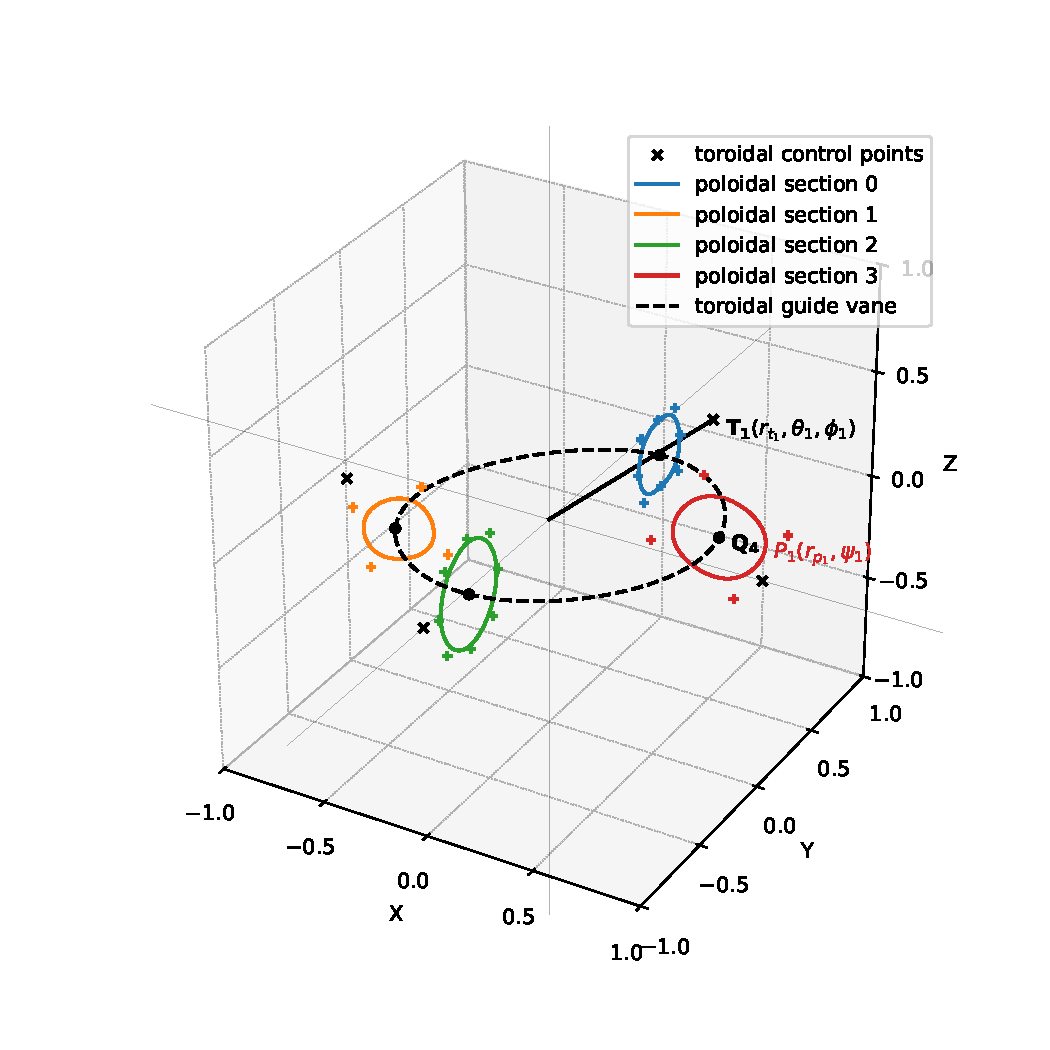
\includegraphics[width=\linewidth,page=1]{typeone_geometry.pdf}
        \caption{}
    \end{subfigure}
    \hfill
    \begin{subfigure}{0.32\textwidth}
        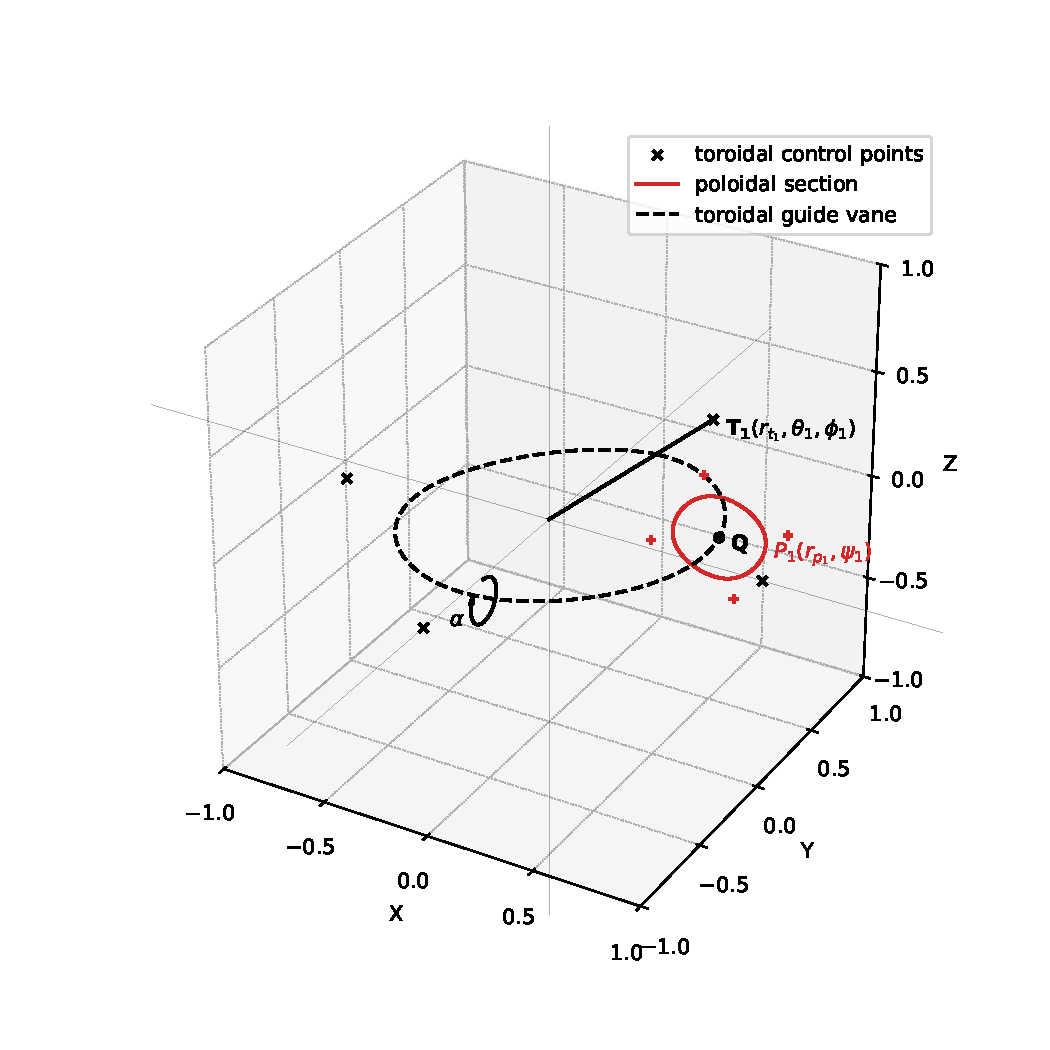
\includegraphics[width=\linewidth,page=1]{typetwo_geometry.pdf}
        \caption{}
    \end{subfigure}
    \hfill
    \begin{subfigure}{0.32\textwidth}
        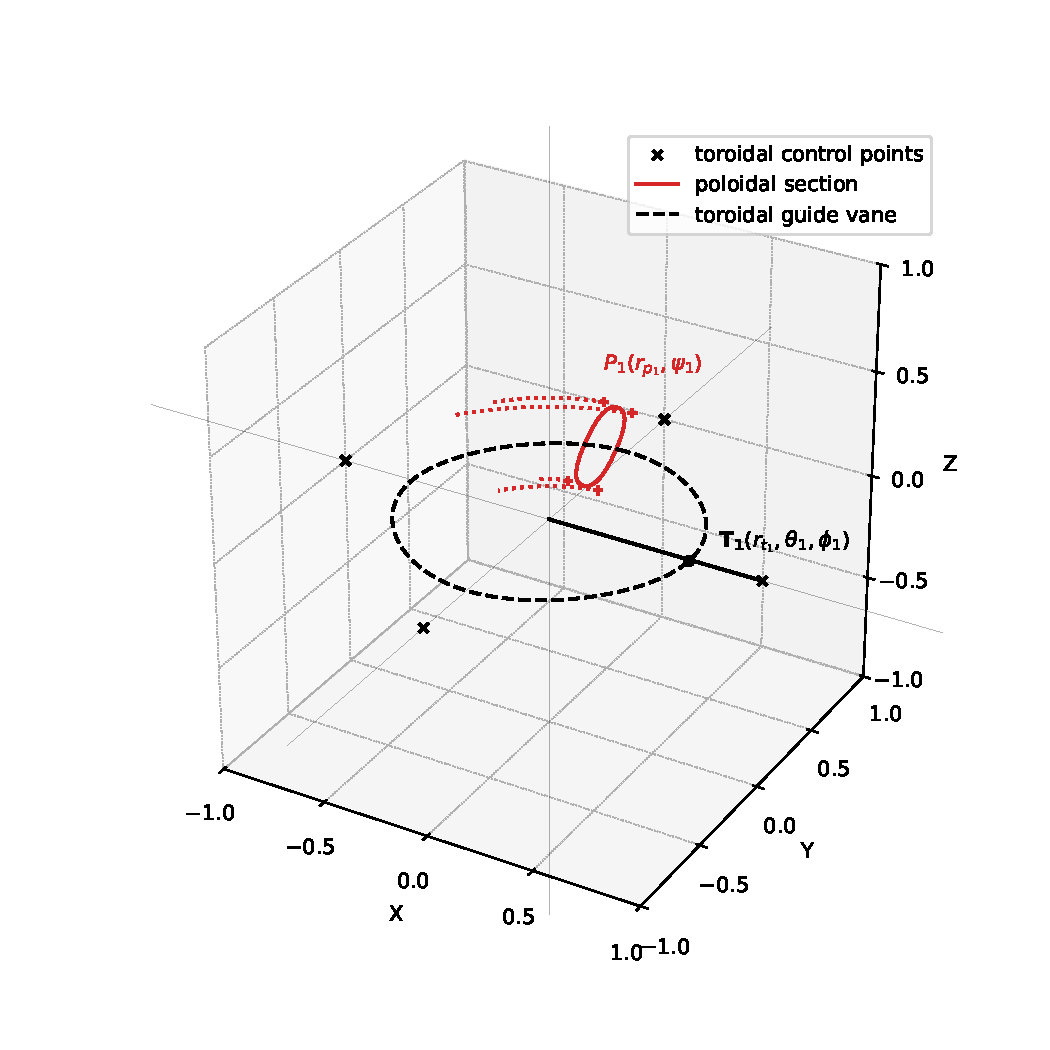
\includegraphics[width=\linewidth,page=1]{typethree_geometry.pdf}
        \caption{}
    \end{subfigure}
    \caption{(a) Type 1 geometry generated with four poloidal cross section $(Q_1,..Q_4)$ definitions and four 3D control points $(T_1,..T_4)$ in spherical coordinate system for 
  the toroidal guide vane. The poloidal section at $Q_4$ consists of four 2D control points in circular coordinate system. Each poloidal section is 
  moved by rotating along the guide vane with its orientation perperndicular to the tangent at that guide vane point. Only $Q_4$ and $T_1$ are depicted.
  (b) Type 2 geoemtry with poloidal section lofted along the 3D toroidal spline with twist parameter $\alpha$ defined along the 3D guide vane.
  (c) Type 3 geometry with spatially varying P($r_p$, $\psi$) along the toroidal guide vane.}
\end{figure}

  \item \textbf{Type 2} - A single poloidal base cross-section is defined using a closed 2D NURBS curve. 
  A twist parameter is then specified along the 3D guide curve. The base cross-section is 
  lofted along the guide vane, while twist and scaling transformations are applied about the local tangential direction.
  \begin{equation}
  \alpha(t) = k \cdot t \cdot \frac{2 \pi}{N} + B \cdot \sin{\frac{N \cdot t \cdot 2 \pi}{P_m}}
  \end{equation}
  The sensitivity of $\alpha$ is given in Appendix \ref{app:twistparam}.
  \item \textbf{Type 3} - The $r_p$ and $\psi$ parameters defining the 2D spline are treated as spatially varying functions along the guide vane.
  \item \textbf{Type 4} - A candidate geometry is represented as 
  the union of N spherical primitives, each defined by its 
  centre coordinates and radius $(x_i, y_i, z_i, r_i)$. 
  The parameters of all spheres form the chromosome used 
  by the genetic algorithm. Geometric variation 
  is achieved by modifying sphere positions and radii, 
  allowing both shape and topology changes during 
  optimisation. Compared with voxel-based encodings, 
  sphere-based representations provide a more compact 
  design space while retaining the ability to represent 
  complex three-dimensional geometries. Similar primitive-based 
  approaches have been used in evolutionary shape 
  optimisation and explicit topology optimisation 
  frameworks such as those of \cite{baron1999voxel} \cite{guo2014mmc}.
\end{itemize}
\begin{figure}[ht]
  \centering
  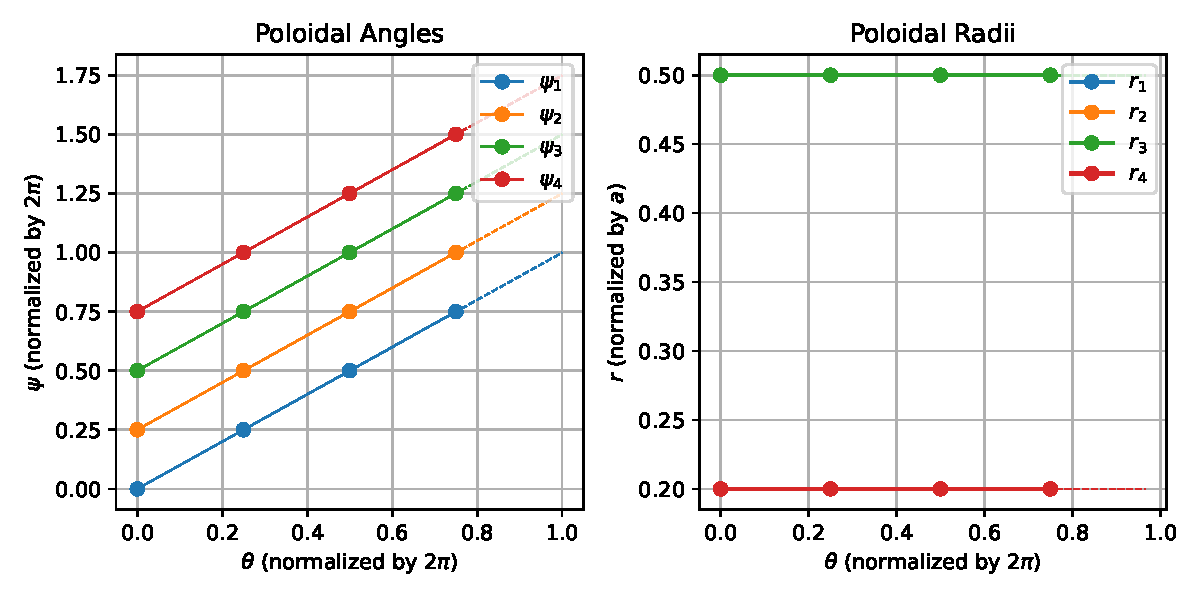
\includegraphics[width=0.7\linewidth,page=1]{poloidal_delta_psi.pdf}
  \caption{Fitting NURBS curve for $\psi$ and $r$ values of Type 3 geometry. Periodic representations
  require the last point to be adjusted accordingly.}
\end{figure}

\section{Optimisation}
A NURBS curve of degree $p$ is defined as:
\begin{equation}\label{equation:nurbs}
\mathbf{C}(u)=
\frac{
\displaystyle\sum_{i=0}^{n} N_{i,q}(u)\, w_i\, \mathbf{P}_i
}{
\displaystyle\sum_{i=0}^{n} N_{i,q}(u)\, w_i
},
\qquad u \in [u_0, u_m].
\end{equation}

The control points $\mathbf{P}_i$ are defined in spherical coordinates and transformed into Cartesian space as
\[
\mathbf{P}_i =
\begin{bmatrix}
r_i \sin\theta_i \cos\phi_i \\
r_i \sin\theta_i \sin\phi_i \\
r_i \cos\theta_i
\end{bmatrix},
\]
\subsection{Gradient based methods}
The following variables are parametrisable:
$(\theta_{t}, \phi_{t}, r_{t}, w_{t})_{\text{N}_\text{t}}$, 
$(s_{t}, \psi_{p}, r_{p}, w_{p})_{\text{N}_\text{p}}$. The objective  
function from Equation \ref{min} is used along with constraint 
equations \ref{constr1} and \ref{constr2} for the non-linear optimisation 
problem. Equation \ref{constr3} is irrelevant as rotational edge transform
is naturally encoded in the poloidal section.
Solutions obtained using \texttt{Scipy} algorithms 
\texttt{SLSQP}, \texttt{L-BFGS-G},
\texttt{COBYLA}, \texttt{COBYQA}, 
\texttt{Nelder-Mead}, \texttt{trust-constr} and \texttt{Powell}
are provided. For \texttt{trust-constr} and \texttt{SLSQP}, constraints are modelled as Non-Linear 
representations while for others it is included as a penalty term in the objective function.

\subsection{Genetic Algorithm}
The genetic algorithm was implemented using the Type 2 geometry 
parameterization. Each individual in the population was 
represented by a chromosome containing the complete set of 
normalized geometry parameters, including toroidal radii, 
poloidal radii, angular coordinates, section spacing parameters, 
and global shaping parameters. Each parameter within the chromosome 
constituted a gene that defined a specific aspect of the geometry.

The initial population was generated using Latin Hypercube Sampling (LHS), 
which provides a more uniform coverage of the design space than purely 
random sampling. Objective history is given in Appendix \ref{app:losshistory}
\begin{figure}[ht]
  \centering
  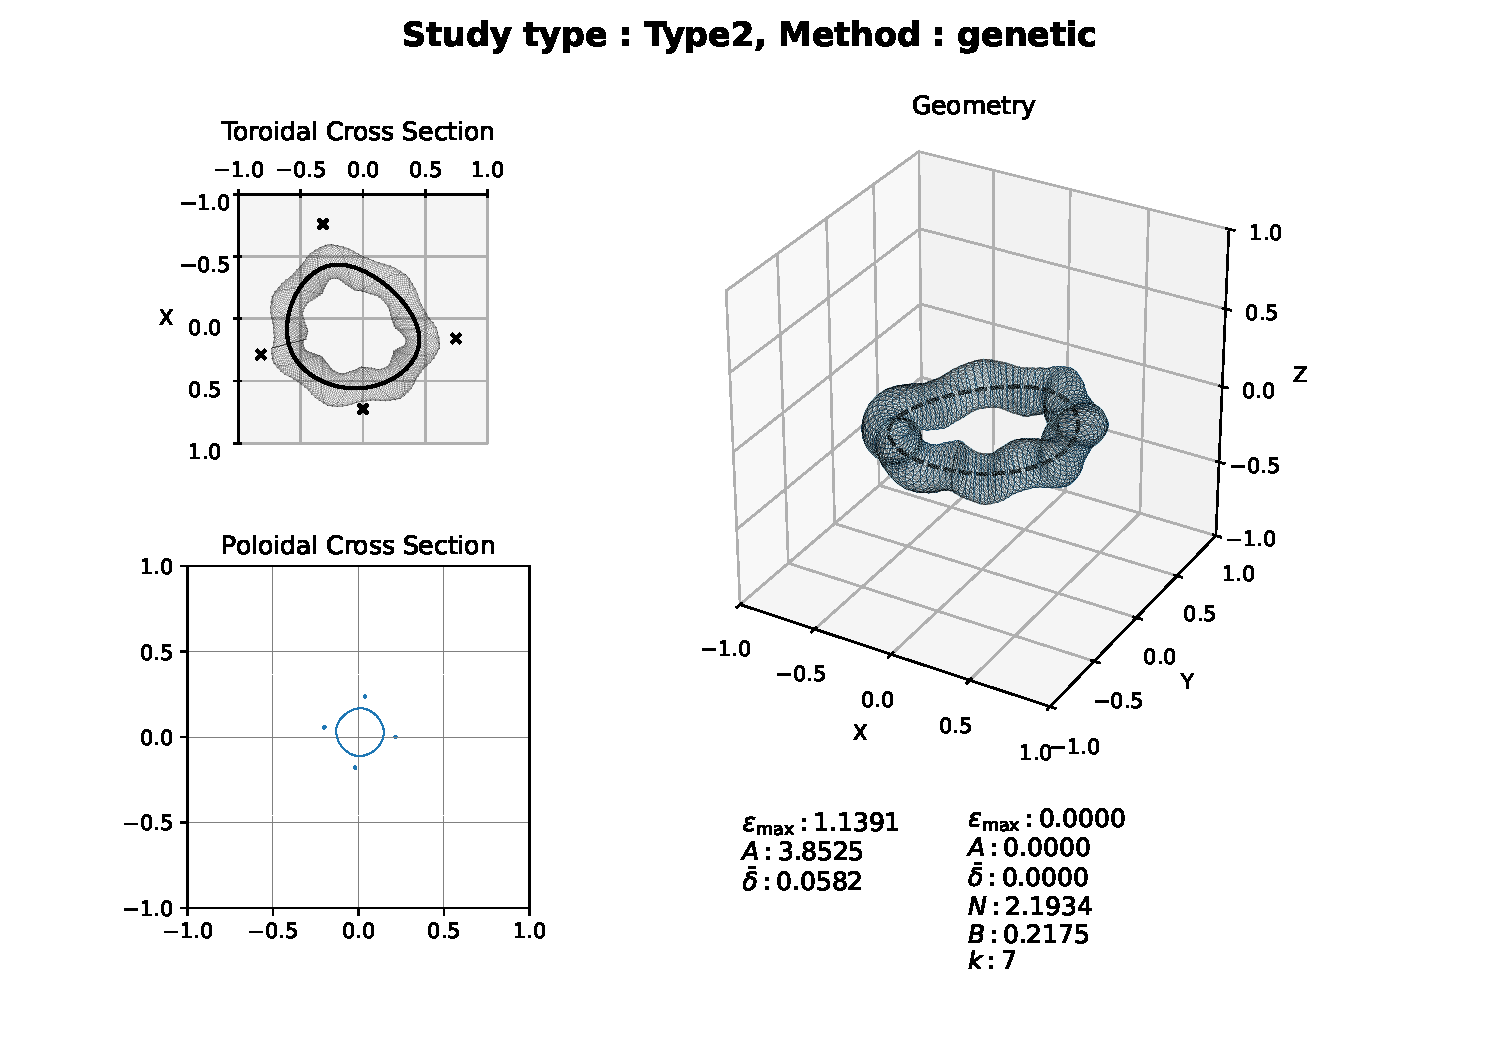
\includegraphics[width=0.7\linewidth,page=1]{Type2_genetic_final_geometry.pdf}
  \caption{Results for Type 2 geometry after 100 generations and an initial 
  population size of 300.}
\end{figure}

\subsection{Neural Networks}

\begin{table}
  \caption{Maximum elongation across different geometry types after optimization using Gradient based methods.}
  \label{scipyoptim}
  \centering
  \begin{tabular}{l|ll|ll|ll}
    \toprule
    & \multicolumn{2}{c|}{Type 1}& \multicolumn{2}{c|}{Type 2}&\multicolumn{2}{c}{Type 3}             \\
    \cmidrule(r){1-7}
    & \multicolumn{2}{c|}{$\epsilon_\text{init}$ = 4.8509}& \multicolumn{2}{c|}{$\epsilon_\text{init}$ = 1.4985}&\multicolumn{2}{c}{$\epsilon_\text{init}$ = 2.6161}             \\
    \cmidrule(r){1-7}
    Optimiser     & \texttt{nfev}     & $\epsilon_\text{max}$ & \texttt{nfev}     & $\epsilon_\text{max}$ & \texttt{nfev}     & $\epsilon_\text{max}$ \\
    \midrule
    L-BFGS-B & 372  & $3.0968$  & 672 & 1.3620 & 69 & 2.6161\\    Nelder-Mead     & 95 & $4.3647$   & 88 & 1.3766 & 70 & 2.6152\\
    Trust-constr     &   186     & $4.7543$  & 64 & 1.4617 & 138 & 1.4992\\
    COBYLA     & 184       & $2.7906$  & 62 & 1.1257 & 136 & 1.7699\\
    COBYQA     & 188       & $3.7076$  & 66 & 1.2460 & 140 & 2.6151\\
    SLSQP     & 283       & $3.5246$  & 101 & 1.1341 & \\
    Powell     &    184    & $4.0724$  & 62 & 1.4957 & 136 & 2.6156\\
    \bottomrule
  \end{tabular}
\end{table}

\subsection*{Acknowledgments}
This research received no specific grant from any funding agency in the public, commercial,
or not-for-profit sectors.

\begin{ack}
This research received no specific grant from any funding agency in the public, commercial, or
not-for-profit sectors.
\end{ack}

\bibliographystyle{plain}
\bibliography{DONUT}


%%%%%%%%%%%%%%%%%%%%%%%%%%%%%%%%%%%%%%%%%%%%%%%%%%%%%%%%%%%%

\appendix

\section{Fourier Geometry}
\label{app:fouriergeom}
\begin{equation}
R(\theta, \phi) = \sum_{n=-N}^{N} \sum_{m=0}^{M} R_{mn} \cos(m \theta - n \text{N}_\text{fp} \phi)
\end{equation}
\begin{equation}
Z(\theta, \phi) = \sum_{n=-N}^{N} \sum_{m=0}^{M} Z_{mn} \sin(m \theta - n \text{N}_\text{fp} \phi)
\end{equation}
%%%%%%%%%%%%%%%%%%%%%%%%%%%%%%%%%%%%%%%%%%%%%%%%%%%%%%%%%%%%

\section{Generations}
\label{app:losshistory}
\begin{figure}[ht]
  \centering
  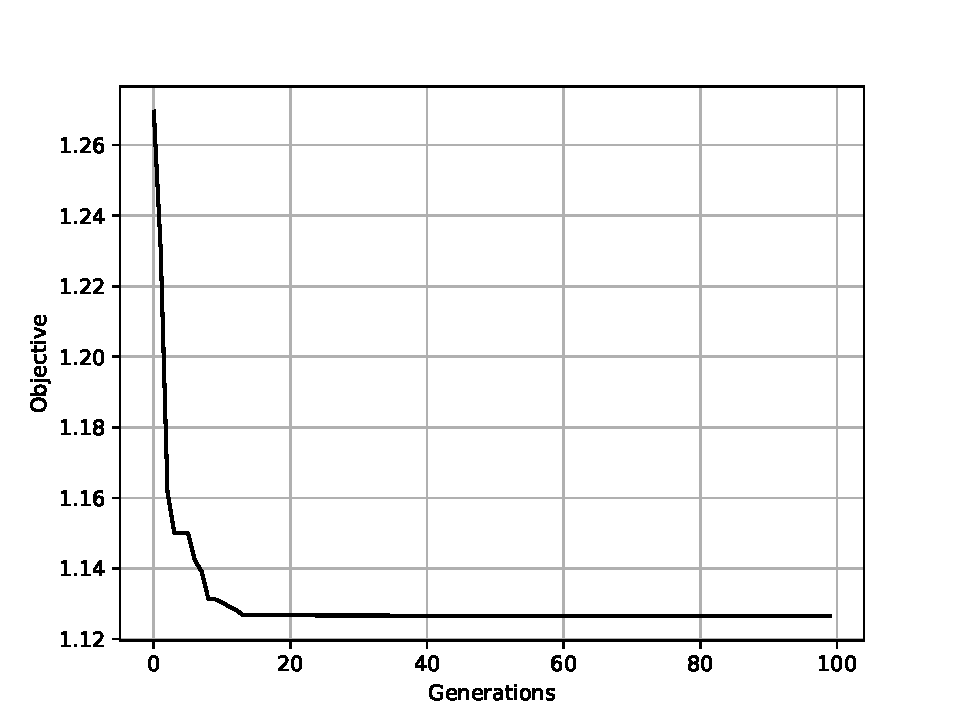
\includegraphics[width=0.4\linewidth,page=1]{loss.pdf}
\end{figure}
\section{Twist parameter}
\label{app:twistparam}
\begin{figure}[ht]
  \centering
  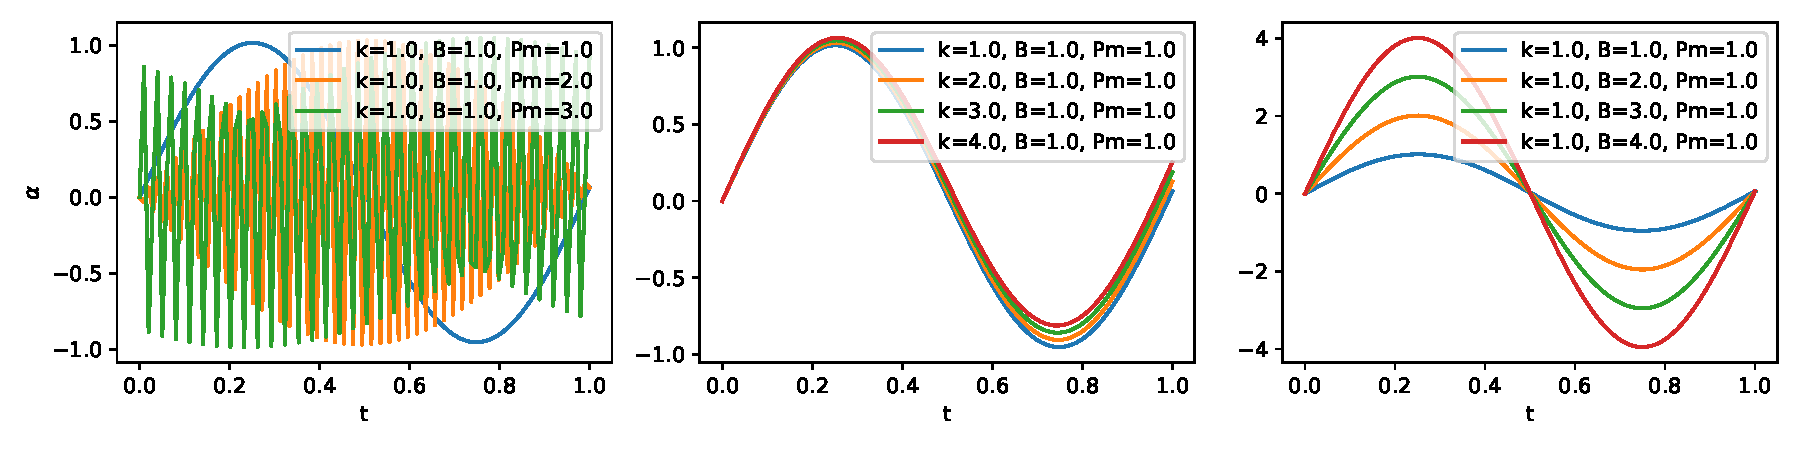
\includegraphics[width=1.0\linewidth,page=1]{Twistparameter.pdf}
\end{figure}
\newpage
% \input{checklist.tex}


\end{document}